This section presents an overview of search-based software test generation and automated crash reproduction and how they are connected to this thesis.

\subsection{Search-based Software Test Generation}
\label{sec:background:unit}
McMinn~\cite{McMinn2004} defined search-based software testing (SBST) as \textit{``using a meta-heuristic optimizing search technique, such as a genetic algorithm, to automate or partially automate a testing task"}.
Within this realm, test data generation at different testing levels (such as \textit{unit testing}, \textit{integration testing}, \etc) has been actively investigated~\cite{McMinn2004}. This section 
provides an overview of earlier work in this area.

\subsubsection{Search-based approaches for unit testing}
SBST algorithms have been extensively used for unit test generation. Previous studies confirmed that thus generated tests achieve a high code coverage~\cite{Panichella2018a, Campos2018}, real-bug detection~\cite{almasi2017industrial}, and debugging cost reduction~\cite{soltani2017, Panichella2016}, complementing manually-written tests.

From McMinn's \cite{McMinn2004} survey about search-based test data generation, we observe that most of the current approaches rely on the control flow graph (CFG) to abstract the source code and represent possible execution flows. The $CFG_m=(N_m,E_m)$ represents a method\footnote{Or function in procedural programming languages.} $m$ as a directed graph of \textbf{basic blocks} of code (the nodes $N_m$), while $E_m$ is the set of the control flow edges. An edge connects a basic block $n_1$ to another one $n_2$ if the control may flow from the last statement of $n_1$ to the first statement of $n_2$. 

Listing~\ref{list:ClassA} presents the source code of \texttt{Person}, a class representing a person and her transportation habits. A \texttt{Person} can drive home (lines 4-10), or add energy to her car (lines~12-18). Figure~\ref{fig:CCFG} presents the CFG of two of Person's methods, with the labels of the nodes representing the line numbers in the code. Since method \texttt{driveToHome} calls method \texttt{addEnergy}, \texttt{node 6} is transformed to two nodes, which are connected to the entry and exit point of the called method. This transformation is explained in the last paragraph of this section.  

\begin{lstlisting}[frame=tb,
    caption={Class \texttt{Person}},
    label=list:ClassA,
    language=java,
    captionpos=t,
    numbers=left,
    belowskip=-2.5em,
    float=t,
    firstnumber=1]
class Person{
    private Car car = new Car();
    protected boolean lazy = false;
    public void driveToHome(){
        if (car.fuelAmount < 100) {
            addEnergy();
        } else {
            car.drive();
        }   
    }

    protected void addEnergy(){
        if (this.lazy) {
            takeBus();
        } else {
            car.refuel();
        }
    }   
    }
  \end{lstlisting}

  \begin{figure}[t]
    \centering
	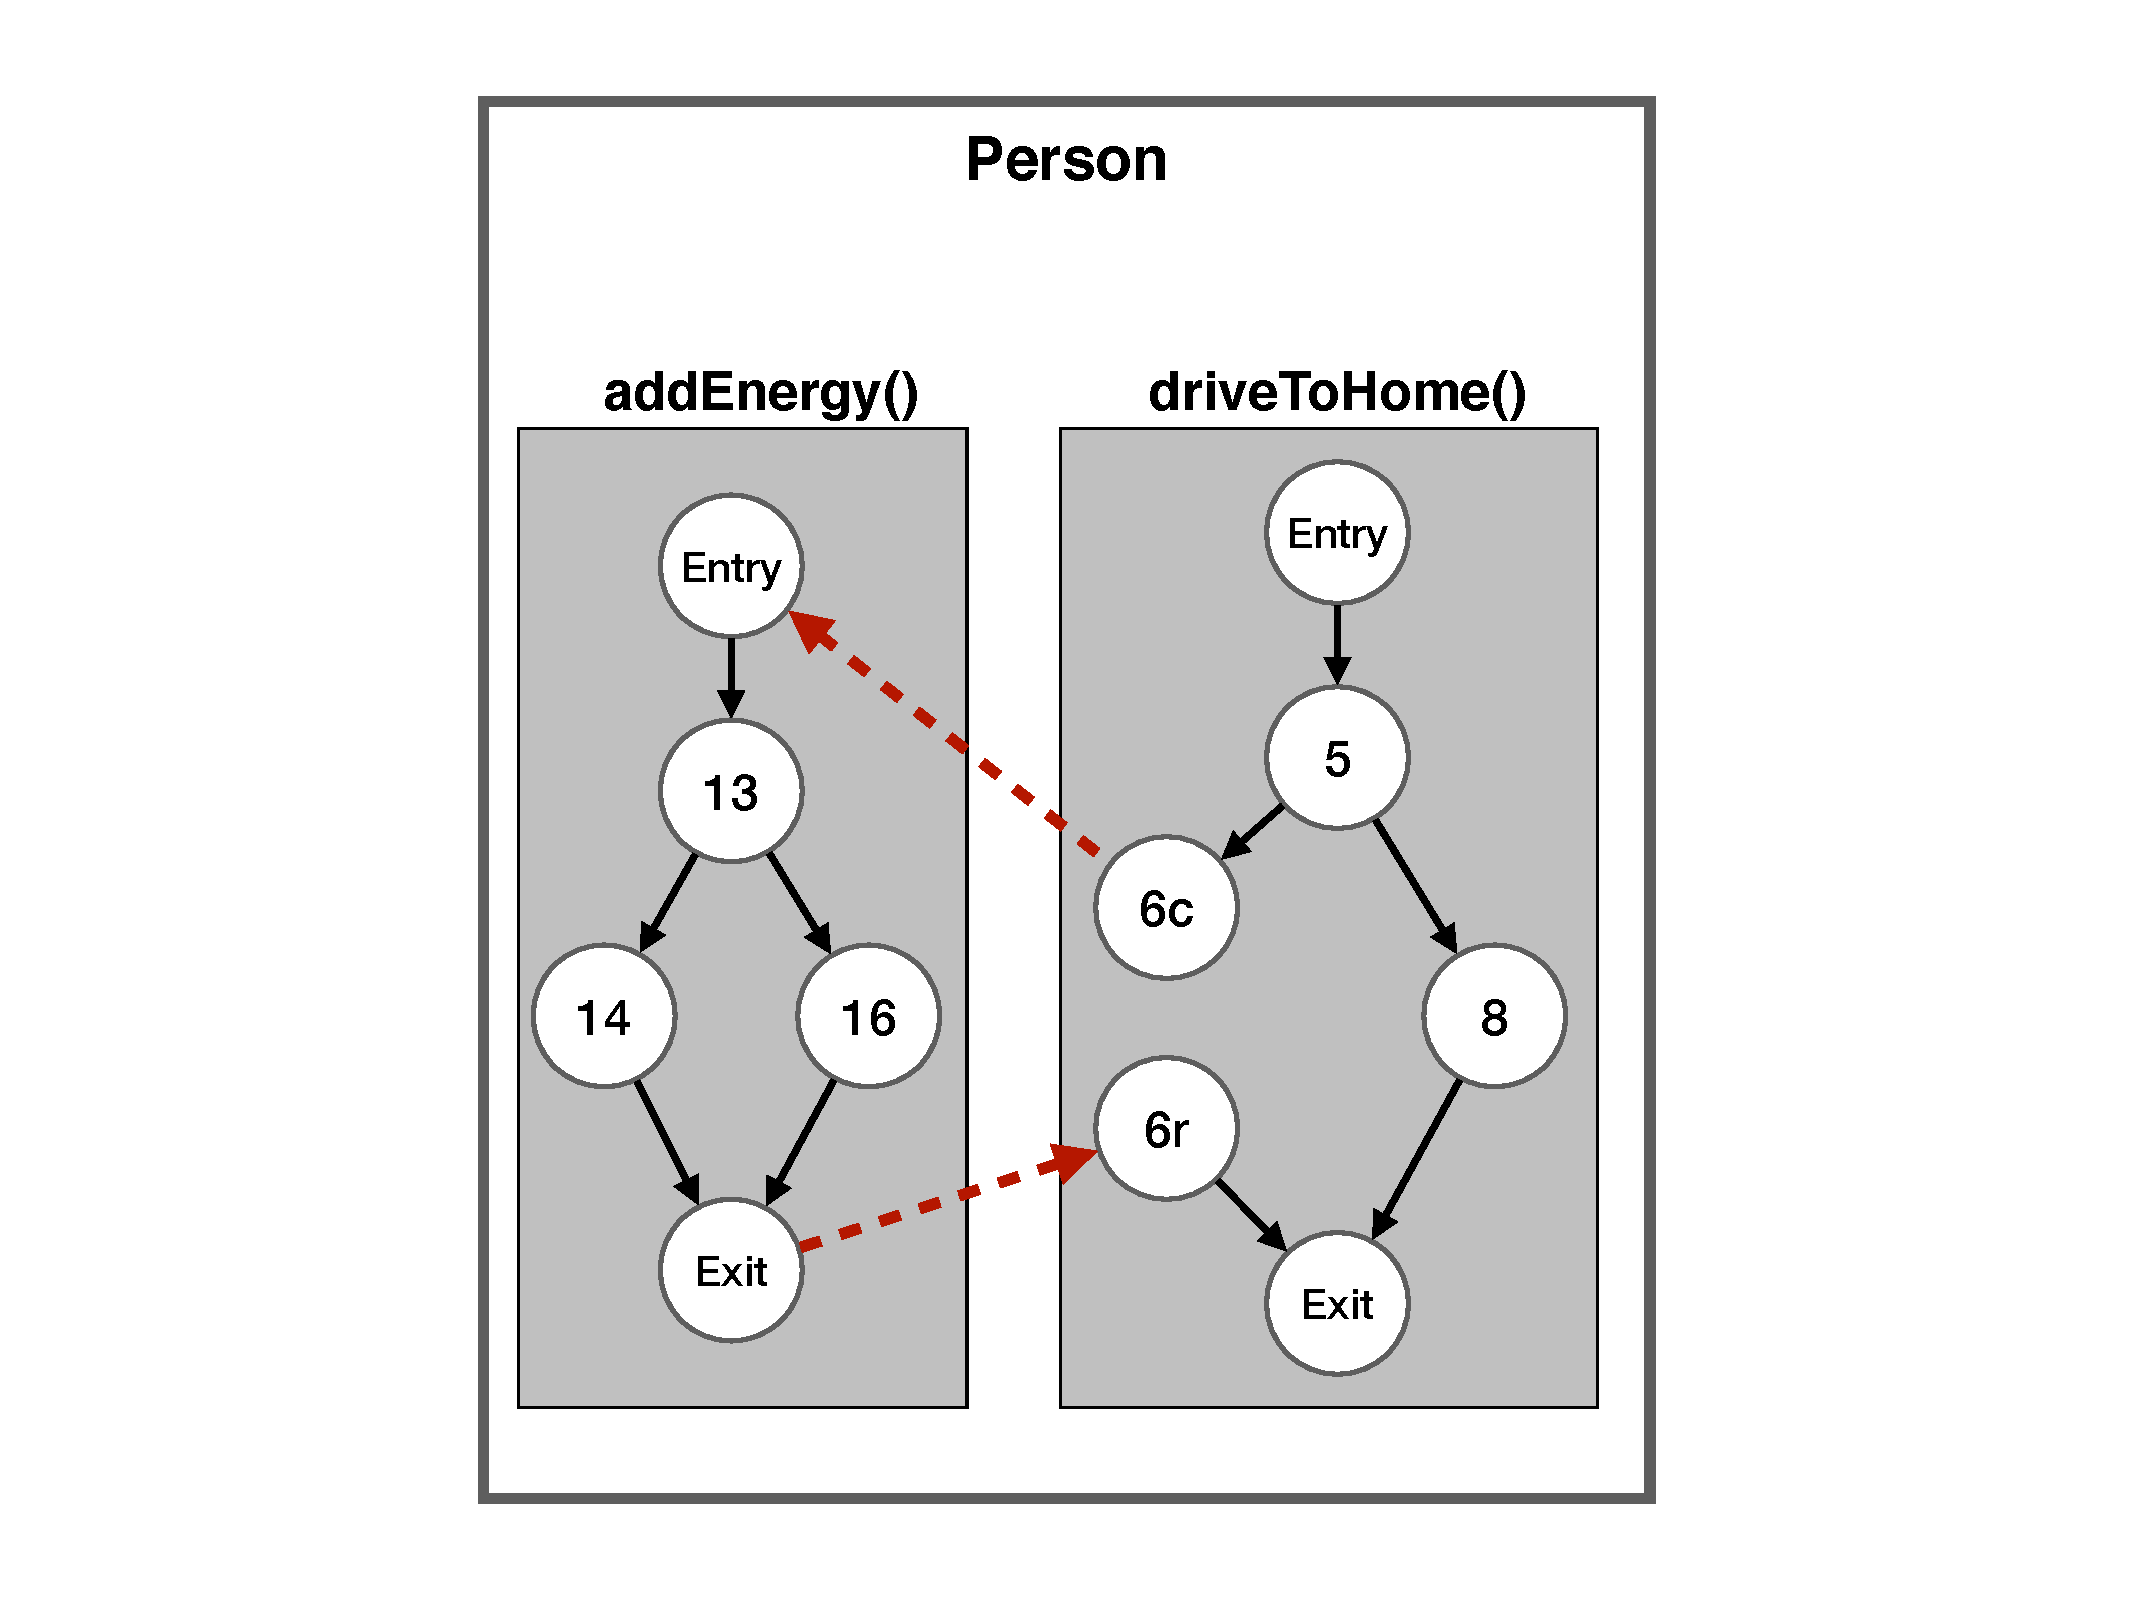
\includegraphics[width=0.85\linewidth]{figs/CCFG_new}
	\caption{Class-level CFG for class \texttt{Person}}
  \label{fig:CCFG}
\end{figure}


Many structural-based approaches combine two common heuristics to reach a high branch and statement coverage in unit-level testing. These two heuristics  are \textit{approach level} and \textit{branch distance}.
The \textit{branch distance} measures (based on a set of rules) the distance to \textit{satisfying} (true branch) and the distance to \textit{not satisfying} (false branch) a particular branching node in the program.
The \textit{approach level} measures the distance between the execution path and a target node in a CFG. To describe how this heuristic measures this distance, we 
rely on the concepts of \textbf{post-dominance} and \textbf{control dependency}~\cite{Allen:1970:CFA:800028.808479}. 

%
As an example, in Figure \ref{fig:CCFG}, \textit{node 8} is control dependent on \textit{node 5} and \textit{node 8} post-dominates edge $\langle 5,8\rangle$. %, but it does not post-dominate $node 5$ itself ($node 5$ can reach the exit point through $node 6$). 
The \textit{approach level} is the minimum number of control dependencies between a target node and an executed path by a test case. 

This thesis leverages the information carved from different resources to introduce search objectives complementing approach level and branch distance for different test generation scenarios. 
% Chapters \ref{sec:jcrashpack:introduction} to \ref{section:bbc:introduction} try to achieve this goal in test generation for on instance of specific behaviors (\ie crash reproduction). Chapter \ref{sec:cling:introduction} uses the call-site information to generate test cases for class integration. Finally, 

\subsubsection{Search-based approaches for integration testing}

Search-based approaches are widely used for test ordering \cite{Wang2010, Steindl2012, Hashim2005, Vergilio2012, Bansal2009, JIiang2019, Borner2009, Mariani2016, Guizzo2015, Abdurazik2009, DaVeigaCabral2010, Briand2003a, Vergilio2012}, typically with the aim of executing those tests with the highest likelihood of failing earlier on. % These studies propose a solution for ordering the integration testing of the classes in the software under test (SUT). However, they do not offer any solution for automated integration test generation.
However, search-based approaches have rarely been used for generating integration tests. Ali Khan \etal \cite{AliKhan2013} have proposed a high-level evolutionary approach that detects the coupling paths in the data-flow graphs of classes and have used it to define the fitness function for the genetic algorithm. Then, the fitness function aids the genetic algorithm to generate tests for the detected coupling paths. Moreover, they proposed another approach for the same goal, which uses Particle Swarm Optimization \cite{Khan2014}. However, the paper does not describe the fitness function and genetic algorithm used in their approach, nor any evaluation for examining the quality of the tests generated by this approach. 
The paper also does not check whether the tests can complement tests generated by existing search-based unit testing approaches. Besides, since objectives are defined according to the def-use paths between classes, the number of search objectives can grow exponentially, thus severely limiting the scalability of the approach.

In Chapter \ref{sec:cling:introduction} we propose a novel approach for class integration test generation.
Instead of using the data flow graph, which is relatively expensive to construct as it needs to find the coupling paths, we use the information available about the the integration between classes to calculate the fitness of the generated tests. Also, we assess our generated tests using different metrics.

\subsubsection{Search-based approaches for other testing levels}

Arcuri \cite{Arcuri2019} proposed EvoMaster, an evolutionary-based white-box approach for system-level test generation for RESTful APIs. A test for a RESTful web service is a sequence of HTTP requests. EvoMaster tries to cover three types of targets:
 \begin{inparaenum}[(i)]
 \item all of the statements in the System Under Test (SUT);
 \item all of the branches in the SUT; and
\item different returned HTTP status codes.
\end{inparaenum}
Although EvoMaster tests different classes in the SUT, it does not systematically target different integration scenarios between classes.

In contrast to EvoMaster, other approaches perform fuzzing \cite{Holler2012}, \textit{``an automated technique providing random data as input to a software system in the hope to expose a vulnerability.''} Fuzzing uses information like grammar specifications \cite{Holler2012, beyene2012, coppit2005, godefroid2008} or feedback from the program during the execution of tests \cite{Padhye2019} to steer the test generation process.
These approaches are black-box and do not rely on any knowledge about classes in the SUT. Hence, their search processes are not guided by the integration of classes.

The approaches introduced in this thesis performs white-box testing.

\subsection{Automated Crash Reproduction}
Software crashes commonly occur in operating environments and are reported to developers for inspection.
When debugging, reproducing a reported crash is among the tasks a developer needs to do in order to identify the conditions under which the reported crash is triggered \cite{Zeller2009, BellerICSE2018}.
In particular, for Java programs, when a crash occurs, an exception is thrown. A developer strives to reproduce it to understand its cause, then fix the bug, and finally add a (non-)regression test to avoid reintroducing the bug in future versions. 

Manual crash reproduction can be a challenging and labor-intensive task for developers: it is often an iterative process that requires setting the debugging environment in a similar enough state as the environment in which the crash occurred~\cite{Zeller2009}.

To help developers in this process, various automated techniques have been suggested.
These techniques can be divided into three categories, based on the kind of data used for crash reproduction: \emph{record-replay approaches} record data from the running program; \emph{post-failure approaches} collect data from the crash, like memory dump; and \emph{stack-trace based post-failure} use only the stack trace produced by the crash. We briefly describe each category hereafter.

\paragraph{Record-replay approaches.}

These approaches record the program runtime data and use them during crash reproduction. The main limitation is the availability of the required data. Monitoring software execution may violate privacy by collecting sensitive data, the monitoring process can be an expensive task for the large scale software, and may induce a significant overhead \cite{Chen2015, Nayrolles2017, Rossler2013}.
%
Tools like \textrm{ReCrash} \cite{Artzi2008}, \textrm{ADDA} \cite{Clause2007}, \textrm{Bugnet} \cite{Narayanasamy2005}, \textrm{jRapture} \cite{Steven2000}, \textrm{MoTiF} \cite{Gomez2016}, \textrm{Chronicler} \cite{Bell2013}, and \textrm{SymCrash} \cite{Cao2014} fall in this category.


\paragraph{Post-failure approaches.}

Techniques from this category use the software data collected directly after the occurrence of a failure. For instance, \textrm{RECORE} \cite{Rossler2013} applies a search-based approach to reproduce a crash by using the stack trace and a core dump, produced by the system when the crash happened, to guide the search.
% Instead, \evocrash only considers the stack trace (usually provided when a bug is reported in an issue tracker) and a distance, similar to the one described by Rossler \etal \cite{Rossler2013}, to guide the search.

Although these tools limit the quantity of monitored and recorded data, the availability of such data still represents a challenge. 
Yu \etal \cite{YZW17descry} addressed this issue for system-level concurrency failure reproduction by introducing \textrm{DESCRY}. 
This approach only uses the default execution logs and applies both static and dynamic analysis combined with symbolic execution to generate the input data and interleaving schedule. 
However, even this approach suffers from two limitations: 
\begin{inparaenum}[(i)]
\item since this tool relies on symbolic execution, applying it on the large and complex projects leads to path explosion;
\item the performance of this tool is strongly linked to the quality of the software log.
\end{inparaenum}
%
Other \textit{post-failure approach} inlcude: Weeratunge \etal \cite{Weeratunge2010}, Leitner \etal \cite{Leitner2007, Leitner2009}, and Kifetew \etal \cite{Kifetew2013, Kifetew2014}.

\paragraph{Stack-trace based post-failure.}

Recent studies in crash reproduction \cite{BPT17concrash,soltani2017,Nayrolles2017,Xuan2015,Chen2015} focuses on utilizing data only from a given crash stack trace to enhance the practical application. 
%
Table~\ref{tab:ant49755} illustrates an example of a crash stack trace from Apache Ant\footnote{ANT-49755: \url{https://bz.apache.org/bugzilla/show_bug.cgi?id=49755} } ~\cite{ant} which is comprised of a crash type (\texttt{java.lang.Null\-Pointer\-Exception}) and a stack of frames pointing to all method calls that were involved in the execution when the crash happened.
From a crash stack frame, we can retrieve information about: the crashing method, the line number in the method where the crash happened, and the fully qualifying name of the class where the crashing method is declared.

\begin{table*}[t]
\centering
\caption{The crash stack trace for Apache Ant-49755.}
\label{tab:ant49755}
\begin{tabular}{c|l}
\multicolumn{2}{l}{java.lang.\textbf{NullPointerException}:}\\
\hline
\textbf{Level} & \textbf{Frame} \\
\hline
1 & \textbf{at} org.apache.tools.ant.util.FileUtils.\textbf{createTempFile}(FileUtils.java:\textbf{888})\\
2 & \textbf{at} org.apache.tools.ant.taskdefs.TempFile.\textbf{execute}(TempFile.java:\textbf{158})\\
3 & \textbf{at} org.apache.tools.ant.UnknownElement.\textbf{execute}(UnknownElement.java:\textbf{291}) \\
\end{tabular}
\end{table*}

The state of the research in crash reproduction \cite{Zamfir2010, jin2012bugredux, BPT17concrash, soltani2017, Nayrolles2017, Xuan2015, Chen2015} aims at generating test code that, once executed, produces a stack trace that is as similar to the original one as possible. They, however, differ in their means to achieve this task. 

\textrm{ESD} \cite{Zamfir2010}, a debugger based on execution synthesis, uses forward symbolic execution and static analysis to reach reproduction. This tool focuses more on concurrency and memory safety bugs.
Similarly, \textrm{BugRedux} \cite{jin2012bugredux} uses forward symbolic execution. \textrm{BugRedux} is a crash reproduction tool for C programs.

Since these two tools rely on forward symbolic execution, they can be applied only on medium-size applications. Also, as illustrated by Braione \etal \cite{braione2017tardis}, symbolic execution test generation approaches face limitations when generating complex input data structures.
To address these limitations, \textrm{STAR} \cite{Chen2015} applies optimized backward symbolic execution and uses a novel technique for method sequence composition to generate a unit test that satisfies the computed preconditions, and eventually reproduces the target crash. 
However, as reported by Chen \etal \cite{Chen2015}, \textrm{STAR} still suffers from the path explosion stemming from utilizing symbolic execution. 
It only supports 3 types of exceptions: explicitly thrown exceptions, \texttt{NullPointerException}, and \texttt{ArrayIndexOutOfBoundsException}.  

\textrm{JCHARMING} \cite{Nayrolles2017} applies model checking to reproduce the reported bugs. To prevent state explosion in the model, it utilizes program slicing.
Since \textrm{JCHARMING} can be applied to any frame from a given crash stack trace, the approach can reproduce any fraction of the target crash stack trace. 

\textrm{MuCrash} \cite{Xuan2015} is based on exploiting existing test cases written by developers and mutating them until they trigger the target crash.
Test case mutation in \textrm{MuCrash} is directed by selecting tests for the classes included in the target crash stack trace. 

Finally, \textrm{Concrash} \cite{BPT17concrash} focuses on reproducing \textit{concurrency} failures that violate thread-safety of a class.
\textrm{Concrash} iteratively generates test code and looks for a thread interleaving that triggers a concurrency crash.
In order to steer the test generation process and avoid expensive computations, \textrm{Concrash} applies the pruning strategies to avoid redundant and irrelevant test code. In contrast with other crash reproduction techniques, \textrm{Concrash} only reproduces the minority of the crashes in the issue tracking systems. As reported by Yuan \etal \cite{Yuan2014}, inter-leaving crashes cause only 10\% of failures in the distributed data-intensive systems. Besides, Coelho \etal \cite{Coelho2015} state that this number is even lower in the Android applications (2.9\%).

\subsection{Search-based Crash Reproduction With \evocrash}

Search-based algorithms have been increasingly used for software engineering problems since they are shown to suite complex, non-linear problems, with multiple optimization objectives that may conflict or competing~\cite{harman12trends}.
\evocrash \cite{soltani2017, Soltani2018a} is a search-based approach to crash reproduction, which applies a \textit{guided genetic algorithm} to search for a unit test that reproduces the target crash. They have shown that this search-based technique outperforms other automated crash reproduction approaches.

\evocrash takes as input a stack trace with one of its frames set as the \emph{target frame}. 
The target frame is composed of 
(i) \emph{target class}, the class to which the exception has been propagated;
(ii) \texttt{target method}, the method in that class; and 
(iii) \emph{target line}, the line in that method where the exception has been propagated. 
It then seeks to generate a unit test that replicates the given stack trace from the target frame (at level $n$) to the deepest frame (at level 1). 
For instance, if we pass the stack trace in Table \ref{tab:ant49755} as the given trace and indicate the second frame as the target frame (level 2), the output of \evocrash will be a unit test for the class \texttt{TempFile} which replicates the first two frames of the given stack trace with the same type of the exception (\texttt{NullPointerException}).

\subsubsection{Guided genetic algorithm}
\label{sec:background:evocrash:guidedalg}
The search process in \evocrash begins by randomly generating unit tests for the target frame.
In this phase, called \emph{guided initialization}, the target method corresponding to the selected frame (i.e., the \emph{failing method} to which the exception is propagated) is injected in every randomly generated unit test.
During subsequent phases of the search, \emph{guided crossover} and \emph{guided mutation}, standard evolutionary operations are applied to the unit tests.
However, applying these operations involves the risk of losing the injected failing method.
Therefore, the algorithm ensures that only unit tests with the injected failing method call remain in the evolution loop. 
If the generated test by crossover does not contain the failing method, the algorithm replaces it with one of its parents. 
Also, if the resulting test does not contain the failing method after a mutation, the algorithm redoes the mutation until the failing method is added to the test again.
The search process continues until either the search budget is over or a crash reproducing test case is found.

To evaluate the generated tests, \evocrash applies the following weighted sum fitness function \cite{Soltani2018a} (called \CrashFunction, hereafter) to a generated test $t$:
%
\rowcolors{1}{}{}
\begin{equation} \label{eq:fitnessfunction}
f(t) = 
\left\{
  \begin{array}{lcr}
    3 \times d_{s}(t) + 2 \times max(d_{except}) + max(d_{trace})   && \textit{if the line is not reached}\\
    3 \times min(d_{s}) + 2 \times d_{except}(t) + max(d_{trace})   && \textit{if the line is reached}\\
    3 \times min(d_{s}) + 2 \times min(d_{except}) + d_{trace}(t)   && \textit{if the exception is thrown}
  \end{array}
\right.
\end{equation}
\rowcolors{1}{}{gray!15}
%
Where:
%
\begin{itemize}
\item $d_{s} \in [0,1]$ indicates the distance between the execution of $t$ and the target statement $s$ located at the target line. 
This distance is computed using the \textit{approach level}, measuring the minimum number of control dependencies between the path of the code executed by $t$ and $s$, and normalized \textit{branch distance}, scoring how close $t$ is to satisfying the branch condition for the branch on which$s$ is directly control dependent \cite{McMinn2004}. 
If the target line is reached by the test case, $d_{l}(t)$ equals to $0.0$;
%
\item $d_{except}(t) \in \{0,1\}$ indicates if the target exception is thrown ($d_{e} = 0$) or not ($d_{e} = 1$);
%
\item $d_{trace}(t) \in [0,1]$ indicates the similarity of the input stack trace and the one generated by $t$ by looking at class names, methods names and line numbers;
%
\item $max(\cdot)$ denotes the maximum possible value for the function.
\end{itemize}
%
Since the stack trace similarity is relevant only if the expected exception is thrown by $t$, and the check whether the expected exception is thrown or not is relevant only if the target line where the exception propagates is reached, $d_{except}$ and $d_{trace}$) are computed only upon the satisfaction of two \emph{constraints}: the target exception has to be thrown in the target line $s$ and the stack trace similarity should be computed only if the target exception is actually thrown. 

Unlike other stack trace similarity measures (e.g., \cite{Rossler2013}), Soltani \etal \cite{Soltani2018a} do not require two stack traces to share the same common prefix to avoid rejecting stack traces where the difference is only in one intermediate frame. Instead, for each frame, $d_{trace}(t)$ looks at the closest frame and computes a distance value. Formally, for an original stack trace $S*$ and a test case $t$ producing a stack trace $S$, $d_{trace}(t)$ is defined as follows:
%
\rowcolors{1}{}{}
\begin{equation}
d_{trace}(t) = \varphi \left( \sum_{f* \in S*} min \left\lbrace \mathit{diff}(f*, f) : f \in S \right\rbrace \right)
\end{equation}
\rowcolors{1}{}{gray!15}
%
Where $\varphi (x) = x / (x+1)$ is a normalization function \cite{McMinn2004} and $\mathit{diff}(f*, f)$ measures the difference between two frames as follows: 
%
\rowcolors{1}{}{}
\begin{equation}
\mathit{diff}(f*, f) = 
\left\{
  \begin{array}{lcr}
    3 && \textit{if the classes are different}\\
    2  && \textit{if the classes are equal but the methods are different}\\
     \varphi \left( \vert l* - l \vert \right)   && \textit{otherwise}
  \end{array}
\right.
\end{equation}
\rowcolors{1}{}{gray!15}
%
Where $l$ (resp. $l*$) is the line number of the frame $f$ (resp. $f*$).

Each of the three components if the fitness function defined in Equation \ref{eq:fitnessfunction} ranges from $0.0$ to $1.0$, the overall fitness value for a given test case ranges from $0.0$ (crash is fully reproduced) to $6.0$ (no test was generated), depending on the conditions it satisfies. 


\begin{table*}[t]
	\centering
	\caption{The number of crashes used in each crash reproduction tool experiment, the gained reproduction by them, and the involved projects.}
	\label{tab:background:represults}
	\small
\begin{tabular}{ l | c c c } 
\textbf{Tool} & \textbf{Reproduced/Total} & \textbf{Rate} & \textbf{Projects} \\
\hline 
\textbf{ EvoCrash~\cite{soltani2017, Soltani2018a}} & 46/54 & 85\% & \begin{tabular}[x]{@{}c@{}}Apache Commons Collections\\Apache Ant \\Apache
Log4j \\ActiveMQ \\DnsJava \\ JFreeChart \end{tabular} \\
%
\textbf{ EvoSuite~\cite{Soltani2018a}}  & 18/54 & 33\% & 
\begin{tabular}[x]{@{}c@{}}Apache Commons Collections\\Apache Ant \\Apache
Log4j \\ActiveMQ \\DnsJava \\ JFreeChart \end{tabular} \\
%
\textbf{ STAR~\cite{Chen2015}} & 30/51 & 59\% &
\begin{tabular}[x]{@{}c@{}}Apache Commons Collections\\Apache Ant \\Apache
Log4j \end{tabular} \\
%
\textbf{ MuCrash~\cite{Xuan2015}} & 8/12 & 66\%  &
\begin{tabular}[x]{@{}c@{}}Apache Commons Collections \end{tabular}\\
%
\textbf{ JCharming\cite{Nayrolles2017}} & 8/12 & 66\% &
\begin{tabular}[x]{@{}c@{}}Apache Ant \\Apache
Log4j \\ActiveMQ \\DnsJava \\ JFreeChart \end{tabular} \\
\end{tabular}
\end{table*}

\subsubsection{Comparison with the state-of-the-art}


\paragraph{Crash reproduction tools.}
%
Table \ref{tab:background:represults} presents the number of crashes used in the benchmarks used to evaluated stack-trace based post-failure crash reproduction tools as well as their crash reproduction rates. 
\evocrash has been evaluated on various crashes reported in other studies and has the highest reproduction rate.

%Unfortunately, as explained by Soltani \etal \cite{soltani2017, Soltani2018a}, other crash reproduction tools are not publicly available, and the reported comparisons in these studies are performed based on results published in \cite{Chen2015, Nayrolles2017, Xuan2015}. 

\paragraph{\evosuite{}.}
%
Table \ref{tab:background:represults} also reports the comparison of \evocrash with \evosuite, using exception coverage as the primary objective, applied by Soltani \etal \cite{Soltani2018a}. All the crashes reproduced by \evosuite could also be reproduced by \evocrash on average 170\% faster and with a higher reproduction rate. 


\subsubsection{Usefulness for debugging}

When reproducing a stack trace with \evocrash, there is no guarantee that the generated test reproduces completely the conditions in which the crash happened in the first place. Besides the random nature of search-based approaches, test cases are generated at the unit level, while crashes usually happen at the system level. However, rather than reproducing the exact same conditions of the crash, the goal of crash reproduction is to help developers fix the underlying bug.

Chen \etal \cite{Chen2015} introduced a usefulness criterion for the crash reproduction approaches. 
According to this criterion, a crash reproducing test is useful to the developers if it covers the buggy frame, \ie if the target frame for which the reproduction is successful is higher than the frame that points to the buggy method.
Soltani \etal \cite{Soltani2018a} refined that criterion through a controlled experiment with 35 master students in computer science and two crashes to assess the degree to which the tests generated by \evocrash helps to debug code. 
Their results indicate that the reproducing tests generated by \evocrash help the participants to fix the bugs more often, although not significantly, and significantly faster. 
They confirmed the usefulness criterion defined by the Chen \etal \cite{Chen2015}, but also found evidence that test cases categorized as not useful can still help developers fix the bug.


